\documentclass[10pt,twocolumn,letterpaper]{article}

\usepackage{iccv}
\usepackage{times}
\usepackage{epsfig}
\usepackage{graphicx}
\usepackage{amsmath}
\usepackage{amssymb}
\usepackage{url}
\usepackage{multirow}
\usepackage{subfigure}
\usepackage{tabularx}

%\linespread{2}
% Include other packages here, before hyperref.

% If you comment hyperref and then uncomment it, you should delete
% egpaper.aux before re-running latex.  (Or just hit 'q' on the first latex
% run, let it finish, and you should be clear).
\usepackage[pagebackref=true,breaklinks=true,letterpaper=true,colorlinks,bookmarks=false]{hyperref}

% \iccvfinalcopy % *** Uncomment this line for the final submission

\def\iccvPaperID{1944} % *** Enter the ICCV Paper ID here
\def\httilde{\mbox{\tt\raisebox{-.5ex}{\symbol{126}}}}

% Pages are numbered in submission mode, and unnumbered in camera-ready
\ificcvfinal\pagestyle{empty}\fi

\begin{document}

%%%%%%%%% TITLE
\title{Abstract Hidden Markov Model for Online Discrete and Continuous Flow Gesture Recognition}

\author{First Author\\
Institution1\\
Institution1 address\\
{\tt\small firstauthor@i1.org}
% For a paper whose authors are all at the same institution,
% omit the following lines up until the closing ``}''.
% Additional authors and addresses can be added with ``\and'',
% just like the second author.
% To save space, use either the email address or home page, not both
\and
Second Author\\
Institution2\\
First line of institution2 address\\
{\tt\small secondauthor@i2.org}
}

\maketitle
%\thispagestyle{empty}

%%%%%%%%% ABSTRACT
\begin{abstract}
We developed an online gesture recognition framework based on abstract hidden Markov  
models (AHMMs). An AHMM closely models the human gesture production process, and its dynamic
Bayesian network (DBN) representation allows for efficient parameter learning and inference
of gestures from observed features. To our knowledge, it is the first application
of AHMM in gesture recognition. We propose a method for handling both continuous and discrete
flow gestures within our inference framework rather than hand-coding the mode switch conditions into the system. 
We compare various inference methods for gesture recognition using our framework and
show that only a small time lag in inference (5 time frames) can increase the recognition
accuracy by 24\% from the result with no time lag, resulting in 82.4\% accuracy. 
Preliminary evaluation also shows that our method can successfully differentiate continuous and discrete flow gestures. 

\end{abstract}

%%%%%%%%% BODY TEXT
\section{Introduction}\label{sec:intro}
With touch-based smart phones and tablets proliferating, people are more and more often 
interacting with computation using their hands. Touch-based interaction feels more
natural because this is how we interact in the real world, using our hands
to manipulate objects and to communicate ideas. Devices like Microsoft's 
Kinect and the Leap Motion Controller
will accelerate this trend by providing even finer hand tracking. 

But understanding the \textit{meaning} of hand movement still remains a challenge because gestures are less constrained and not
easily described in a grammar. There are also different kinds of gestures, each of which may 
require slightly different treatment from the system. Wobbrock \etal developed a taxonomy of surface gestures based on a user-defined
gesture set~\cite{Wobbrock09}, classifying each gesture along four dimensions: 
\textit{form}, \textit{nature}, \textit{binding}, and \textit{flow}. \textit{Flow} is particularly relevant from a system development
point view because it refers to how the system should respond to users' acts. 
There are two categories in this dimension: \textit{discrete} and 
\textit{continuous}. A gesture's \textit{flow} is discrete if the system response
should occur \textit{after} the user acts; it is continuous if the system response
should occur \textit{while} the user acts~\cite{Wobbrock09}. Their user-elicited
gesture set of 1080 gestures from 20 participants was evenly split between discrete and continuous flow 
gestures.

In this paper we consider gesture recognition fundamentals (i.e., understanding the gesture production process and developing a model for it), and 
gesture recognition pragmatics (i.e., developing a 
the system that responds correctly and promptly). We discuss the 
details of gesture modeling in Section~\ref{sec:gesture-modeling}. Based on that, in Section~\ref{sec:ahmm}, we detail 
our abstract hidden Markov model based framework for online gesture recognition and a way to
handle continuous and discrete flow gestures. We show our experimental results in Section~\ref{sec:eval}.

\subsection{Related work}
Previous work on gesture recognition has focused on discrete flow gestures of either
static (hand is held in one location) or dynamic (hand moves) forms \cite{suryanarayan10, song12}. Hidden Markov models (HMMs) are commonly used
to recognize this type of gesture~\cite{Starner95}. 
One HMM model is trained for each gesture class, resulting in a mixture of HMMs~\cite{yin10} . During
recognition, a segmented gesture sequence is presented to each HMM and the one that gives the highest
likelihood of the observed sequence determines the gesture class. 

Some researchers have used discriminative models (e.g., hidden conditional 
random fields (HCRF)~\cite{wang06}, or latent-dynamic conditional random fields (LDCRFs)~\cite{morency07}), which can provide some 
performance improvement over an HMM. But HCRFs
can only handle segmented gesture sequences and LDCRFs can only handle bounded sequences. Song \etal~\cite{song12} extend the LDCRF by 
adding exponential smoothing to the prediction at each time frame, but their model does not
use the end state of each gesture as a constraint to the gesture transition, and thus, may not
model the gesture production process adequately.  

Fran\c coise applied a 2-level hierarchical hidden Markov model (HHMM) for real-time 
gesture segmentation and recognition~\cite{francoise10}, but used a limited gesture set and basic features (e.g., accelerometer readings).
AHMMs and HHMMs are closely related, and both of them have been used to model user activities~\cite{nguyen03, nguyen05}. Our
evaluation compared 2 variations from the models based on our gesture data set.

Prior work on handling both discrete and continuous flow gestures have been limited and 
usually involve explicit mode change on the user's part. Oka \etal developed a 
system that distinguishes a gesture as either continuous or discrete (in their 
terms ``manipulative'' or ``symbolic'') according to the extension of the 
thumb~\cite{Oka02}: gestures with an extended thumb were interpreted as direct manipulation,
 those with a bent thumb as symbolic gestures. For direct manipulation, the
system selects operating modes such as rotate, move or resize, based on the fingertip
configuration; for symbolic gestures, it uses HMM for classification. The use of
an explicit thumb position to distinguish the two types of gestures is clearly not natural behavior.

As a general issue Wobbrock \etal found, users rarely care about the number of fingers they 
employ~\cite{Wobbrock09}, which is at odd with many designer-defined gesture sets
~\cite{Malik05, Morris06, Rekimoto02, Tse06}. Other mode change methods may have the
user perform a grab gesture to start the continuous flow mode and a release gesture
to end it. In the photo browsing system developed by Madhvanath \etal~\cite{Madhvanath12},
users use two hands to start the zoom action, whereupon the system switches to continuous
mode, allowing users to pan the photo as well. This seems more natural but may still
be limited and constrained. 

\section{Gesture modeling} \label{sec:gesture-modeling}
We first describe our model of gesturing, which provides the foundation for choices we
make in the design of our system. 

\subsection{Gesture production}
The production and perception of gestures 
can be modeled in a way similar to that done in spoken language recognition~\cite{Pavlovic97}.
Gestures originate as a gesturer's mental concept, and are expressed through the motion of arms and 
hands. Observers perceive gestures as streams of visual images, which they
interpret using their knowledge about those gestures. In gesture recognition, the 
observer is the computer and the knowledge it possesses is the training data we 
give it.

\subsection{Gesture flow}
To respond properly, the system must differentiate discrete and continuous
flow gestures. If a gesture's flow
is discrete, the whole sequence needs to be delimited, recognized, and responded
as a single event. For example, a \textit{wave} gesture that can mean ``no'' or getting the attention of the 
system should be responded at the end of the gesture. On the other hand, if the 
flow is continuous, ongoing system response is required. Consider the \textit{pan} and the \textit{resize} gestures, 
as the user moves his/her hand(s), the system has to respond in each frame such that
certain parameter(s) of the virtual object(s) that the user is controlling are tied to
certain parameter(s) of the user's hand(s).

One major distinction between discrete and continuous flow gestures is that,
in a pre-defined gesture set, discrete flow gestures usually have specific hand
poses and movement paths, where continuous flow gestures usually do not have
specific movement paths and the hand poses are not as strictly defined. For
example, when panning, the user's hand may move in any
direction. As a result, 
 we cannot train the system with examples of  the
\textit{pan} gesture in only one direction.

Our approach has
one class for all the continuous flow gestures and different classes for the different
discrete flow gestures. The training data for the continuous flow gesture class
should be examples of gestures moving in different directions to account for the 
variability in this class. 

\subsection{Temporal modeling of gestures}
Previous research suggests that
a gesture consists three phases: preparation, nucleus 
(also called peak or stroke~\cite{Mcneil82}), and retraction~\cite{Pavlovic97}. The preparation phase consists
of a preparatory movement that sets the hand in motion from some resting position.
The nucleus of a gesture has some ``definite form and enhanced dynamic qualities''
~\cite{kendon86}. Finally, the hand either returns to the resting position or repositions
for the new gesture phase. 

Most previous work for recognizing discrete flow gestures does not
distinguish the preparation and retraction phases (citations) from the rest of the gesture
sequence (Sharma \etal~\cite{sharma00} is an exception). While it may not be necessary to treat the preparation
and retraction phases separately for discrete flow gestures, we believe it is 
necessary for continuous flow gestures, because
the system needs to respond immediately when the nucleus of a continuous flow
gesture starts, but not during the preparation and retraction. As a result, we have one class for the preparation phase and one class for the 
retraction phase, explicitly modeling each, so that we can detect
the start and end of the nucleus phase of the continuous gesture. 

We can use a hierarchical hidden Markov model (HHMM)~\cite{fine98} to describe the combination of the 
gesture production and temporal model. Figure~\ref{fig:hhmm} shows an example of 
this generative process. A gesture phase state is an ``abstract state'' which 
calls its hand/arm movement sub-HMM. The hand/arm movement sub-HMM can have self-loops 
and skip transitions to represent variable duration of gestures. When a sub-HMM
reaches the end state, it returns control to wherever it was called from. The 
hand/arm movement states are ``production states'' which emit single observations. 

\begin{figure}[h]
  \centering
  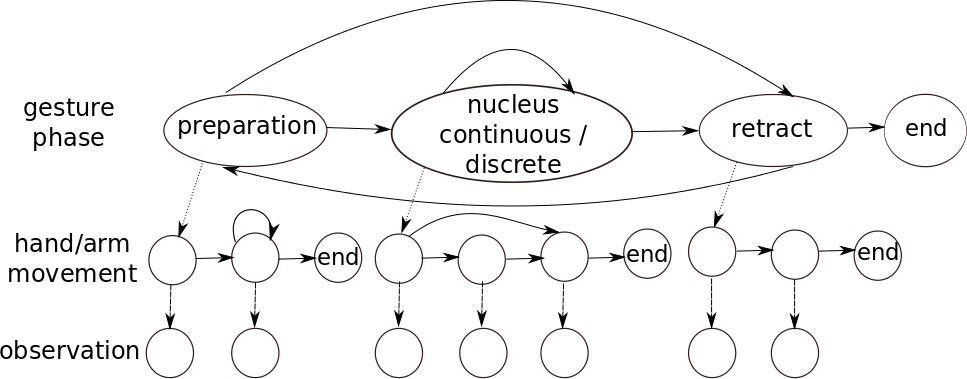
\includegraphics[width=0.5\textwidth]{figure/hhmm.png} 
  \caption{State transition diagram for a 2-level HHMM representing the gesture
  production process. The transitions shown are for illustration purpose and do not
  necessary reflect the actual state transitions in the model.}
  \label{fig:hhmm}
\end{figure}

\section{AHMM based framework for online gesture recognition} \label{sec:ahmm}
The abstract hidden Markov model (AHMM) proposed by Bui \etal~\cite{bui00} maps closely to the
gesture production model. It is also closely related to HHMMs. The authors are interested
in inferring what goal an agent currently has by observing its effect in the world. Translated
to our gesture recognition problem: we want to infer the user's intended gesture (his/her goal), based on observations captured by the sensor.  

The AHMM models the end state of the sub-HMMs. A sub-HMM ends when the upper level
goal is satisfied. Using an AHMM, we can model the gesture phases and segment the start and end of the nucleus phase of the gesture
so that the system can respond promptly. 

While it is possible to consider a multi-level AHMM to represent a gesturer's goal at
different levels of abstraction, we start by considering the simplest case first, i.e.,
a 1-level AHMM~\cite{bui01}. Figure~\ref{fig:ahmm} shows a 1-level AHMM represented
as a dynamic Bayesian network (DBN)~\cite{murphy02}. Representing an AHMM in a DBN allows us to use efficient algorithms to do learning
and online inference. For details about DBNs, see~\cite{murphy02}.

In our gesture recognition framework,
$G_t$ represents the gesture phase that the
gesturer has at time $t$. It includes the preparation phase ($P$), the retraction phase ($R$), 
the nucleus phase with continuous flow ($NC$), and various nucleus phases with discrete flow ($NC_i$). $S_t$ is the hidden
state of the hand movement, which is essentially a vector quantization of the actual, observed 
(but noisy) feature vector $X_t$. $F_t^G$ is a binary indicator variable that is
``on'' (has value 1) if the lower level HMM at time $t$ has just ``finished''
(i.e., is about to enter an end state), otherwise it is ``off'' (value 0).

The AHMM DBN shown in Figure~\ref{fig:ahmm} is defined by a set of conditional probability distributions (CPD) which
includes
\begin{align}
P(G_1 = i) &= \text{prior for } G \label{eq:cpd-g1} \\ 
P(S_1 = j | G_1 = i) &= \text{prior for } S \\
P(G_t = j| G_{t - 1} = i, F_{t - 1}^G = f) &= 
\begin{cases}
  \delta(i, j), & \text{if} f = 0 \\
  A^G(i, j), & \text{if} f = 1 
\end{cases} \\
P(F_t^G = 1 | G_t = g, S_t = i) &= A_g^S(i, \text{end}) \\
P(S_t = j | G_{t - 1} = g, S_{t - 1} = i) &= A_g^S(i, j) \label{eq:cpd-s}\\
P(X_t = x_t | S_t = i) &= N(x_t; \mu_i, \Sigma_i). \label{eq:cpd-x}
\end{align}
Here, $\delta(i, j) = 1$ if $i == j$ and $0$ otherwise, and $A^Q_q(i, j)$ is the
transition probability for node $Q$ from state $i$ to $j$ when its parent is $q$.
Since $G_t$, $S_t$ and $F_t$ take discrete values, CPD(\ref{eq:cpd-g1})-(\ref{eq:cpd-s})
can be represented in table forms. $X_t$ take continuous vector values and CPD(\ref{eq:cpd-x})
is a Gaussian distribution.

\begin{figure}[tb]
  \centering
  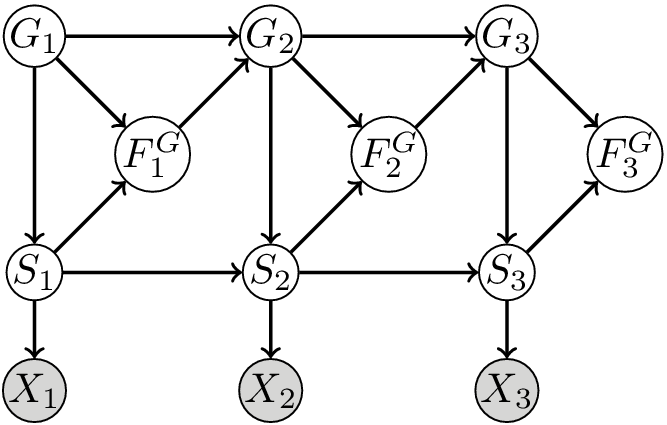
\includegraphics[width=0.4\textwidth]{figure/ahmm.png} 
  \caption{A 1-level AHMM without reset of $S$ state.}
  \label{fig:ahmm}
\end{figure}

One difference between this 1-level AHMM and a general HHMM is that state $S$ never
``resets'', since $F^G$ is not a parent. Here we assume that during a gesture sequence, even if the goal changes,
the next state of the hand/arm movement always depends on the previous state. This is reasonable for gesture recognition because the hand/arm 
movement is always continuous, unless the hands move out of the sensor's view during
which the inference engine will reset. 

Figure~\ref{fig:ahmm-reset} shows an alternative model we evaluated in which
 $S$ does reset when the goal changes. With this model, when $S_t$ resets, the prior
probability $P(S_t = j | G_t = i)$ is used instead of the transition probability. 

We compare the classification accuracy of these two models in Section~\ref{sec:exp-model}.

\begin{figure}[tb]
  \centering
  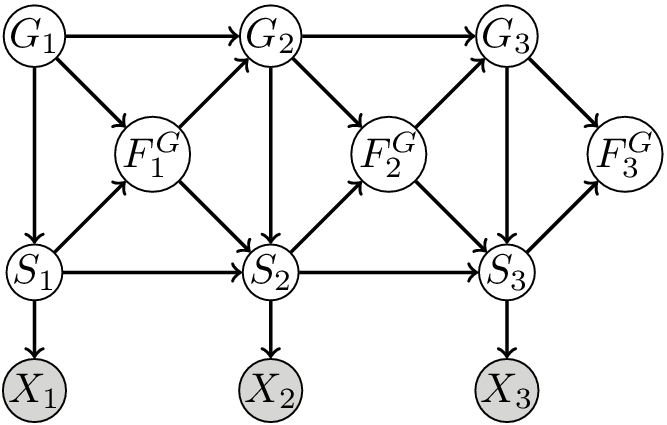
\includegraphics[width=0.4\textwidth]{figure/ahmm-reset.png} 
  \caption{A variant of HHMM with reset of $S$ state.}
  \label{fig:ahmm-reset}
\end{figure}

\subsection{Tabletop environment}
We have experimented with our gesture recognition framework using a custom tabletop 
interface (Figure~\ref{fig:setup}). It includes four $1280\times1024$ pixel 
projectors providing a $2560\times2048$ pixel resolution display. The display is 
projected onto a flat white surface digitizer. The projected displays
were aligned to produce a single seamless large display area using ScalableDesktop\texttrademark Classic software~\footnote{\url{http://www.scalabledisplay.com/products/software/scalabledesktopclassic}}. 
One Microsoft Kinect motion sensor is placed above the center of the
tabletop among the projectors. The Kinect streams $640\times 480$ pixels of
RGB and depth video at about 30 frames per second (fps). 

\begin{figure}[tb]
  \centering
  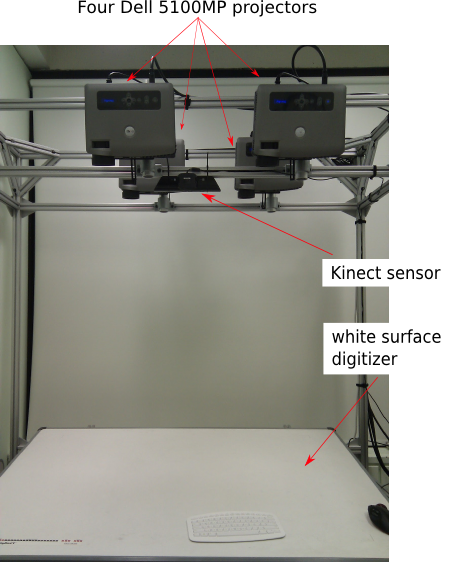
\includegraphics[width=0.34\textwidth]{figure/setup2.png} 
    \caption{System setup.} \label{fig:setup}
\end{figure}

\subsection{Feature extraction}
The feature vector at each time frame $X_t$ includes: 
\begin{itemize}
  \item $d$, perpendicular distance from the centroid of the hand cloud, $\bf{p}\in\mathcal{R}^3$, to the plane of the tabletop 
  \item $\bf{p}_y$, distance from the centroid of the hand point cloud to the center horizontal line of the table
  \item $d\bf{p}\in\mathcal{R}^3$, velocity of the hand
  \item $d^2\bf{p}\in\mathcal{R}^3$, acceleration of the hand
  \item $\boldsymbol{\theta}\in\mathcal{R}^3$, roll, pitch, yaw of the hand
  \item $\bf{h}$, hand pose features vector 
\end{itemize}
Currently we consider only single hand gestures

Our background subtraction is fairly straight forward because the background is the tabletop, which is relative simple and static. As a
result, we use an averaging method, which estimates the plane of the tabletop by computing the average and average difference of each pixel in the depth image.
One iteration of morphological opening is then used to clear out small pixel noise. 
Connected components are found by considering all all contours that are greater than the minimum
length of a hand.
These components are considered to be the hand and the arm and are approximated with convex hulls and bounding boxes. 
The hand region is at either end of the bounding box depending on the position of the arm relative to the table.

Once the bounding box for the hand is found, we use CAMSHIFT~\cite{Bradski98}
to further remove outliers. We then compute the centroid of the hand cloud. We also compute
the major and minor axes using Principle Component Analysis (PCA). We rotate the hand
so that its major axis aligns with the x-axis. This rotation also gives us $\boldsymbol{\theta}$.
We also scale the hand point cloud into a $100$mm cube, with the centroid of the hand 
at the center of cube. Hand pose features are computed
based on this rotational and scale invariant hand point cloud.

\begin{figure}[tb]
  \centering
  \subfigure[depth mapped image]{
    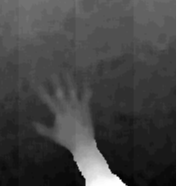
\includegraphics[width=0.25\columnwidth]{figure/depth.png}
    \label{fig:key-adaptive}
  } ~
  \subfigure[bounding box for the hand]{
    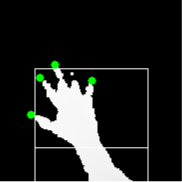
\includegraphics[width=0.26\columnwidth]{figure/hand.png}
    \label{fig:one-finger}
  }
  \subfigure[rotational and scale invariant point cloud]{
    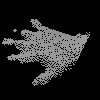
\includegraphics[width=0.26\columnwidth]{figure/normalized.png}
    \label{fig:two-thumb}
  }
  \caption{Image processing steps.}
  \label{fig:key-boundary}
\end{figure}

\subsubsection{Eigenhand features}  
Inspired by the eigenface technique~\cite{turk91}, researchers have applied a similar idea to hand tracking~\cite{asaari12},
hand pose recognition~\cite{Malassiotis08}, and identity verification~\cite{tantachun06}. We apply
this idea for dynamic gesture recognition by including the hand pose features as
part of the feature vector.

Previous work on hand pose recognition is typically focused on a defined set of hand poses, so
labeling the training data set is relatively easy. This is also true for the work on dynamic gesture recognition~\cite{song12}.
Previous work has also used feature descriptors such as HOG, and classification algorithms such as SVM~\cite{song12}.

However, in a more natural setting, there are times where the hand poses are not 
very well defined or salient, for example during preparation and retraction phases.
It is hard to manually define a set of possible hand poses for a such dynamic sequence
of gestures. Given our AHMM model, we need to find hand pose features that can be
viewed as continuous values that can be quantized into a mixture of Gaussians model.

We suggest that Eigenhand may be an reasonable choice because the features are basically 
coordinates in the new space spanned by the eigenhand basis vectors. In this way, the
new features are similar to the other continuous features such as position, velocity
and acceleration.  
 
Given training sequences of hand point clouds, we first convert each point cloud
into a $100 \times 100$ matrix where the x and y coordinates of each point are mapped to the column and 
row of the matrix and the z coordinate is the value. Any point that does not exist in
the hand point cloud has value 0. We use the standard eigenface technique to compute
the eigenhands (i.e. eigenvectors, Figure~\ref{fig:eigen-hand}) from the training data and use the first 3 eigenhands,
$u_1, u_2, u_3$, as our basis. Hence, the hand pose feature vector $\bf{h}$ is a 3-dimensional vector
$[w_1, w_2, w_3]$ where each component is the projection of the hand into each $u_1, u_2, u_3$.
Combined with the rest features, we have a 14-dimensional feature vector
as $X_t$.

\begin{figure}[h]
  \centering
  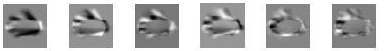
\includegraphics[width=0.5\textwidth]{figure/eigen-hand.png} 
  \caption{First 6 eigenhands.}
  \label{fig:eigen-hand}
\end{figure}

\subsection{Learning}
We use semi-supervised training to learn the parameters (i.e., CPDs, Eq. (\ref{eq:cpd-g1})-(\ref{eq:cpd-x})) of the 1-level AHMM DBN model.
The training data has $G_t$ and $X_t$ observed, but $S_t$ and the finish status, $F_t^G$ are hidden.
We use the junction tree algorithm to do exact inference and the expectation maximization (EM)
algorithms to learn the parameters. 

The result of EM depends on good initialization. As we model the production probability $P(X_t | S_t)$ as a Gaussian distribution, we
can view $X_t$ as a mixture of Gaussians. The number of states $S_t$ can take is the
number of mixtures (i.e., clusters). Through clustering analysis of the training data and
using the Bayesian information criterion~\cite{fraley12}, we found that the best mixture model has 11 clusters
with untied diagonal covariance matrices. So we set the number of state for $S_t$
to be 11, and initialize $\mu_i$ to be the cluster centers. 

\subsection{Inference}
There are different kinds of inference one can perform on a DBN. For online gesture
recognition, to make the system the most responsive, we need to do \textit{online filtering} which is to recursively estimate the
belief state~\cite{murphy02} using the forward algorithm and find the optimal gesture phase
at time $t$ as:
\begin{align*}
g^* &= \arg\max_g P(G_t = g | x_{1:t}) \\
\end{align*}

However, there can be a trade-off between responsiveness and accuracy. If we allow some lag $L$,
we can use more evidence to estimate the gesture phase of past at $t - L$ as:
\begin{align*}
g^* = \arg\max_g P(G_{t - L} = g | x_{1 : t} )
\end{align*}
This is traditionally called ``\textit{fixed-lag smoothing}'' and can often give higher
accuracy. The online filtering is a special case when $L = 0$.

The other extreme is the offline case, where the whole sequence of length $T$ is known. In this case
we can compute the optimal gesture phase for each time frame $t$ as:
\begin{align*}
g^* = \arg\max_g P(G_t = g | x_{1 : T}).
\end{align*}
This is also called ``\textit{fixed-interval smoothing}'' and should give an 
upper bound in gesture recognition for the model.

Another inference method is \textit{Viterbi decoding} which computes the most likely
sequence given the data:
\begin{align*}
g^*_{1:t} = \arg\max_{g_{1:t}}P(g_{1:t} | x_{1:t})
\end{align*}
It can be both online and offline, and is the same as the forwards pass of filtering, 
except we replace sum with maximum~\cite{murphy02}. As our gesture recognition task is
concerned with inferring the most current gesture phase instead of the most probable gesture 
sequence, Viterbi decoding may not be a good choice for inference, because 
taking only the maximum probability loses some information and may make the result 
less robust. 

Given the frame rate and human reaction time, we may allow a few frames of lag in order
to achieve better accuracy. Section~\ref{sec:comp-inf} shows the experimental comparison of different
inference methods.

%------------------------------------------------------------------------
\section{Experimental Evaluation}\label{sec:eval}
Most public gesture data sets have only discrete flow gestures, and usually do not have
segmentation for the start and end of the nucleus phase of gestures. As a preliminary evaluation
of our gesture recognition framework for handling both continuous and discrete flow gestures, 
we collected gesture data from 3 users. Each user performs a series of gestures 
including both continuous and discrete gestures. The continuous gestures include
panning to the right and left, rotating clockwise and anticlockwise. Each is repeated once. 
The discrete gestures include thumb up, stop, and wave; each is repeated three times. 
Overall there are 13 sequences per user, with an average length of 53 frames per
sequence, resulting in a total of 2114 frames. Each sequence contains a preparation phase, a nucleus phase and a retraction
phase.

The users perform the gestures following an example shown to them. The order of the gestures performed is random. 
We manually label the gesture phase class of all the sequences to obtain ground truth.
The gesture phase classes include P (preparation), R (retraction), NC (nucleus-continuous),
ND1 (nucleus-discrete-stop), ND2 (nucleus-discrete-thumbup) and ND3 (nucleus-discrete-wave). Segmenting the gesture
phases manually is rather difficult, as also noted by \cite{francoise10}. Hence
the ground truth segmentation has to be taken with a grain of salt.  

We perform user
dependent training and recognition. The result will be relevant for building a system that can
recognize user-dependent gesture input after the user supplies a few examples of 
each gesture.

All results below are based on 10-fold cross-validation on each user's data; average validation results
are reported. We used the Bayes Net Toolbox for Matlab \footnote{\url{https://code.google.com/p/bnt/}} to implement the training
and inference of the AHMM DBN.

\subsection{Model comparison}\label{sec:exp-model}
We compare the two models mentioned in Section~\ref{sec:ahmm}. In the 1-level AHMM (Figure~\ref{fig:ahmm}), the state $S_t$ does not reset when
the upper level gesture ends; in the
variant of HHMM (Figure~\ref{fig:ahmm-reset}), the state $S_t$ resets. Table~\ref{tab:comp-model} shows the frame-based classification
results using the two models. Fixed-interval smoothing is used during inference.
The result shows that resetting the $S_t$ state gives a worse result, confirming our 
intuition that since hand/arm movement is continuous, it should always depend on
the previous state. 

\begin{table}[tb]
\begin{center}
\begin{tabularx}{0.5\textwidth}{|X|c|c|c|c|}
\hline
\multirow{2}{*}{Model} & \multicolumn{4}{c|}{Frame classification \% accuracy (std.)} \\
\cline{2-5}
      & User 1 & User 2 & User 3 & Average \\
\hline\hline
not reset & 80.4 (19) & 83.3 (18) & 91.7 (7) & 85.1 (15) \\ 
reset & 68.1 (27) & 80.2 (23) & 86.7 (21) & 78.3 (24) \\
\hline
\end{tabularx}
\end{center}
\caption{Comparison of two AHMM models. In the first one, $S_t$ does not reset when the 
gesture completes, and in the second one, $S_t$ does reset. }
\label{tab:comp-model}
\end{table}

\subsection{Inference method comparison} \label{sec:comp-inf}
Using the model in which $S_t$ does not reset, we compare the frame-based
classification result for different inference methods. Table~\ref{tab:comp-inf}
shows that online filtering gives the lowest classification accuracy results as
expected. However, once we add a lag of 5 frames, the accuracy increases to 82.4\%,
a 24\% improvement. 

The result for fixed interval Viterbi decoding is also lower than that of 
smoothing which confirms our intuition. Figure~\ref{fig:comp-inf}
further illustrates the promising result that a small time lag in estimating the 
gesture phase can result in a large improvement in accuracy. Given that our frame 
rate is about 12fps after feature extraction without any optimization, 5 frames is about 0.4s. Further performance optimization
to increase the frame rate and better fine tuning of the recognition model can even push the lag time
some what lower.

\begin{table}[tb]
\begin{center}
\begin{tabularx}{0.5\textwidth}{|l|c|}
\hline
Inference method & \multicolumn{1}{p{0.44\columnwidth}|}{\centering{Frame classification \% accuracy (std.)}} \\
\hline\hline
Online filtering (L = 0) & 66.4 (17) \\
Fixed-lag smoothing (L = 5) & 82.4 (15)  \\
Fixed-lag smoothing (L = 10) & 83.4 (14) \\
Fixed-lag smoothing (L = 20) & 83.8 (15) \\
Fixed interval smoothing & 85.1 (15)  \\ 
Fixed interval Viterbi & 82.5 (11)  \\ 
\hline
\end{tabularx}
\end{center}
\caption{Comparison of frame-based classification accuracy with different inference methods.}
\label{tab:comp-inf}
\end{table}

\begin{figure}[tb]
\begin{center}
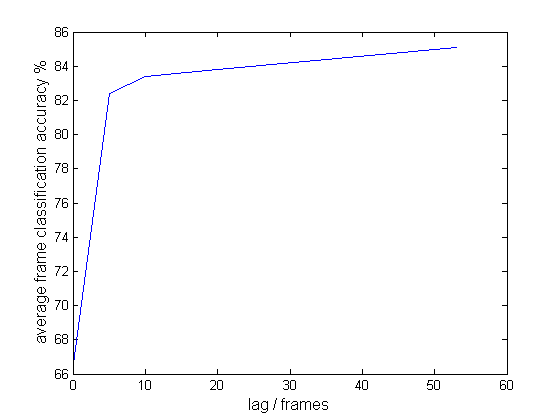
\includegraphics[width=0.5\textwidth]{figure/comp-inf.png}
\end{center}
   \caption{Plot of average frame-based classification \% accuracy agains frame
   lag in estimation.}
\label{fig:comp-inf}
\end{figure}

\subsection{Gesture phase detection}
Using fixed-lag smoothing inference with $L = 5$, we compute the frame-based confusion matrix
between the ground truth gesture phases and the predicted ones. Figure~\ref{fig:confusion-matrix} shows that most gesture phase classification errors
occur between the preparation / retraction phase and the other nucleus phases. This may
partly be due to the time lag in estimation. An example of such delay is shown in Figure~\ref{fig:gesture-phase}.
The example shows a gesture sequence with a continuous flow nucleus phase. The delay of 
the start of nucleus phase is 10 frames while the delay of the end the nucleus phase is about 2 frames.

There is also no confusion between the continuous flow nucleus phase and the other discrete flow
nucleus phases. This suggests that, given a gesture set where the continuous flow gestures
have some features that make them distinguishable from the discrete flow gestures, the framework
can learn these features through examples, instead of having to hand-code them. 

\begin{figure}[tb]
\begin{center}
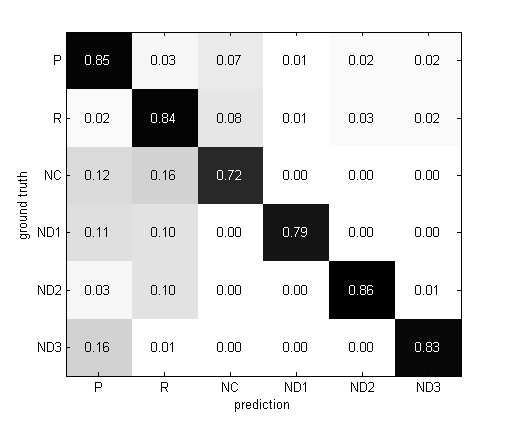
\includegraphics[width=0.5\textwidth]{figure/confusion-matrix.png}
\end{center}
   \caption{Confusion matrix of ground truth gesture phase vs.
   predicted gesture phase for each frame. }
\label{fig:confusion-matrix}
\end{figure}

\begin{figure}[tb]
\begin{center}
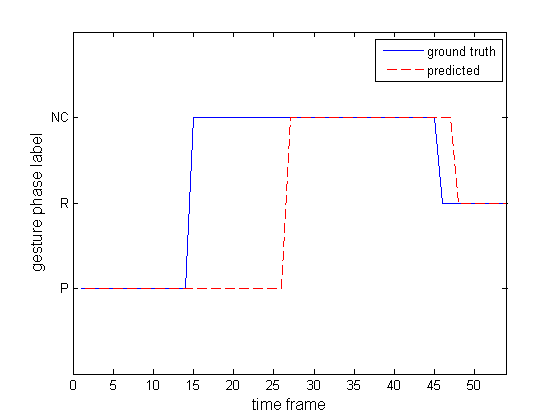
\includegraphics[width=0.5\textwidth]{figure/segmentation.png}
\end{center}
   \caption{Plot of ground truth gesture phase labeling (blue line) and the predicted gesture phase (red dashed line).
   Inference is done with fixed-lag smoothing with $L = 5$.}
\label{fig:gesture-phase}
\end{figure}
  
%------------------------------------------------------------------------
\section{Conclusion and Future Work}
Based on the foundation of gesture modeling, we proposed an abstract hidden Markov model
based framework for online gesture recognition. An AHMM closely models the gesture production process
and the DBN representation allows us to do efficient learning and online estimation. 
Our preliminary evaluation shows promising results for online gesture recognition
with a small amount of time lag. We also proposed a way to handle both continuous and discrete flow gestures in a unified
way based on the inference framework. Our results show that this is a promising method. 

We will evaluate our system with some larger public datasets (even those with just discrete flow gestures) to compare
the results. We will also conduct user-independent evaluations and add user adaptation to our model.
Furthermore, we want to evaluate and compare different hand pose features such as HOG features with the eigenhand features we are using now.

We also plan to implement the framework in a realtime system
to create a testbed for various user studies, including comparing a hard coded mode switching interface to
an inference-based mode switching interface.

{\small
\bibliographystyle{ieee}
\bibliography{egbib}
}

\end{document}
